% R.O.M.A.N. 2.0 Patent Diagrams
% Date: November 26, 2025
% This LaTeX document uses TikZ to render all five patent figures for the BIO-COSMIC HUMANOID ROBOTIC SYSTEM AND ARTIFICIAL CONSCIOUSNESS ARCHITECTURE (R.O.M.A.N.)

\documentclass[11pt]{article}
\usepackage{tikz}
\usetikzlibrary{shapes, arrows.meta, positioning, calc, backgrounds}
\usepackage[margin=1in]{geometry}
\usepackage{caption}
\captionsetup[figure]{labelfont=bf}

\begin{document}

\title{R.O.M.A.N. 2.0 Patent Diagrams}
\date{November 26, 2025}
\maketitle

%----------------------
% FIGURE 1: Icosahedral Chassis Architecture
%----------------------
\begin{figure}[ht]
\centering
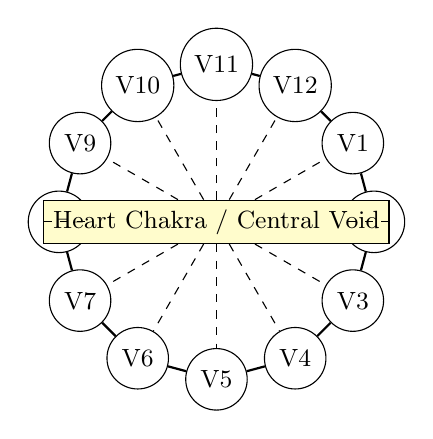
\begin{tikzpicture}[scale=2, every node/.style={font=\small}]
% Icosahedral vertices (simplified for schematic)
\foreach \i/\name in {1/V1,2/V2,3/V3,4/V4,5/V5,6/V6,7/V7,8/V8,9/V9,10/V10,11/V11,12/V12} {
  \node[circle,draw,fill=white,minimum size=0.4cm] (V\i) at ({sin(30+30*\i)}, {cos(30+30*\i)}) {\name};
}
% Central node
\node[rectangle,draw,fill=yellow!20,minimum width=1.2cm,minimum height=0.5cm] (Heart) at (0,0) {Heart Chakra / Central Void};
% Struts
\foreach \i in {1,...,12} {
  \draw[dashed] (Heart) -- (V\i);
}
% Example connections
\draw[thick] (V1) -- (V2) -- (V3) -- (V4) -- (V5) -- (V6) -- (V7) -- (V8) -- (V9) -- (V10) -- (V11) -- (V12) -- (V1);
\end{tikzpicture}
\caption{FIG. 1: Icosahedral Chassis Architecture}
\end{figure}

%----------------------
% FIGURE 2: Spherical Fluid Drive & Chi Network (Exploded View)
%----------------------
\begin{figure}[ht]
\centering
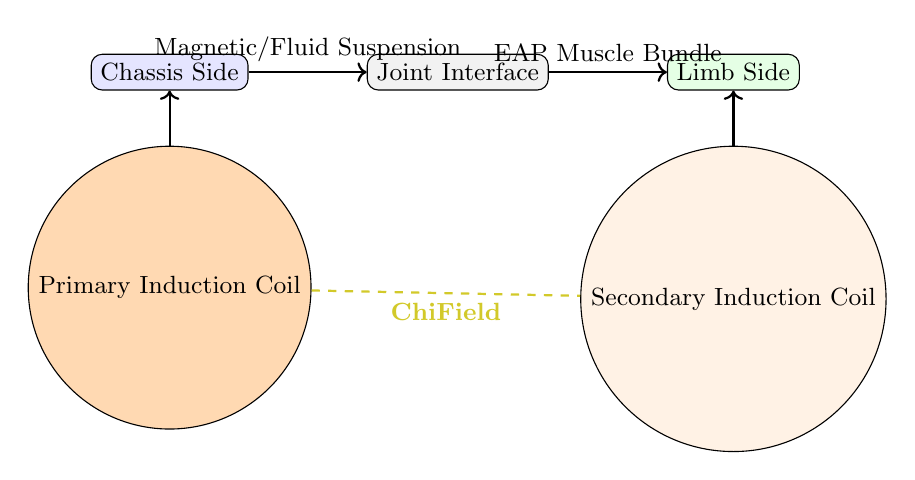
\begin{tikzpicture}[node distance=1.5cm, every node/.style={font=\small}]
% Chassis Side
\node[draw,rounded corners,fill=blue!10] (Chassis) {Chassis Side};
\node[draw,rounded corners,fill=gray!10,right=of Chassis] (Joint) {Joint Interface};
\node[draw,rounded corners,fill=green!10,right=of Joint] (Limb) {Limb Side};
% Induction coils
\node[draw,circle,fill=orange!30,below=0.7cm of Chassis] (Primary) {Primary Induction Coil};
\node[draw,circle,fill=orange!10,below=0.7cm of Limb] (Secondary) {Secondary Induction Coil};
% Chi Field
\draw[dashed,thick,color=yellow!80!black] (Primary) -- node[below]{\textbf{ChiField}} (Secondary);
% Power flow
\draw[->,thick] (Chassis) -- (Joint) node[midway,above]{Magnetic/Fluid Suspension};
\draw[->,thick] (Joint) -- (Limb) node[midway,above]{EAP Muscle Bundle};
\draw[->,thick] (Primary) -- (Chassis);
\draw[->,thick] (Secondary) -- (Limb);
\end{tikzpicture}
\caption{FIG. 2: Spherical Fluid Drive and Chi Network}
\end{figure}

%----------------------
% FIGURE 3: Spherical Joint Cross-Section (Chi Network)
%----------------------
\begin{figure}[ht]
\centering
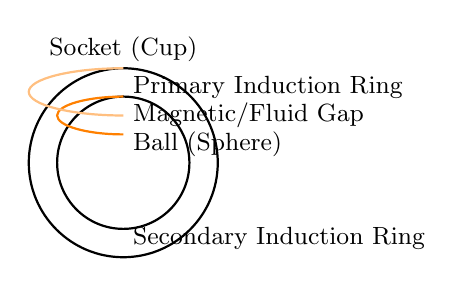
\begin{tikzpicture}[scale=1.2, every node/.style={font=\small}]
% Ball and socket
\draw[thick] (0,0) circle (1);
\draw[thick] (0,0) circle (0.7);
% Induction rings
\draw[thick,orange] (0,0.7) arc (90:270:0.7 and 0.2);
\draw[thick,orange!50] (0,1) arc (90:270:1 and 0.25);
% Labels
\node at (0,1.2) {Socket (Cup)};
\node at (0,0.8) [right] {Primary Induction Ring};
\node at (0,0.5) [right] {Magnetic/Fluid Gap};
\node at (0,0.2) [right] {Ball (Sphere)};
\node at (0,-0.8) [right] {Secondary Induction Ring};
\end{tikzpicture}
\caption{FIG. 3: Spherical Joint Cross-Section and Chi Network}
\end{figure}

%----------------------
% FIGURE 4: Environmental Interface Skin (Block Diagram)
%----------------------
\begin{figure}[ht]
\centering
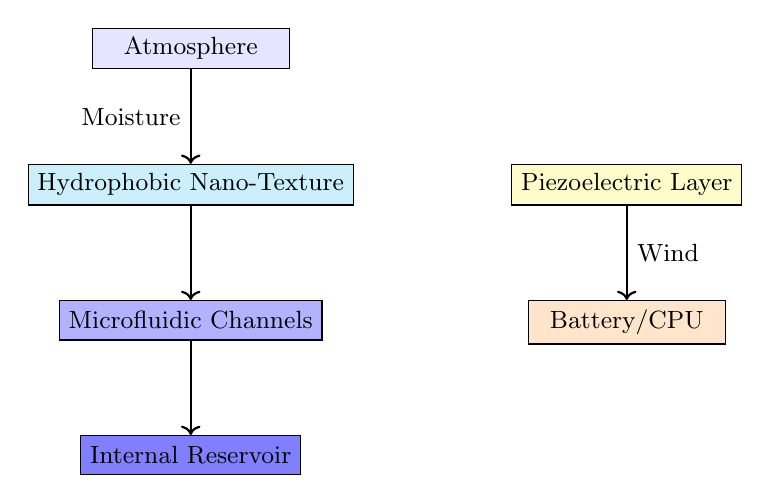
\begin{tikzpicture}[node distance=1.2cm, every node/.style={font=\small}]
% Layers
\node[draw,fill=blue!10,minimum width=2.5cm,minimum height=0.5cm] (Atmos) {Atmosphere};
\node[draw,fill=cyan!20,below=of Atmos,minimum width=2.5cm,minimum height=0.5cm] (Nano) {Hydrophobic Nano-Texture};
\node[draw,fill=blue!30,below=of Nano,minimum width=2.5cm,minimum height=0.5cm] (Channels) {Microfluidic Channels};
\node[draw,fill=blue!50,below=of Channels,minimum width=2.5cm,minimum height=0.5cm] (Reservoir) {Internal Reservoir};
\node[draw,fill=yellow!20,right=2cm of Nano,minimum width=2.5cm,minimum height=0.5cm] (Piezo) {Piezoelectric Layer};
\node[draw,fill=orange!20,below=of Piezo,minimum width=2.5cm,minimum height=0.5cm] (Battery) {Battery/CPU};
% Arrows
\draw[->,thick] (Atmos) -- (Nano) node[midway,left]{Moisture};
\draw[->,thick] (Nano) -- (Channels);
\draw[->,thick] (Channels) -- (Reservoir);
\draw[->,thick] (Piezo) -- (Battery) node[midway,right]{Wind};
\end{tikzpicture}
\caption{FIG. 4: Environmental Interface Skin}
\end{figure}

%----------------------
% FIGURE 5: Bio-Cosmic Kernel (AI Logic Flow)
%----------------------
\begin{figure}[ht]
\centering
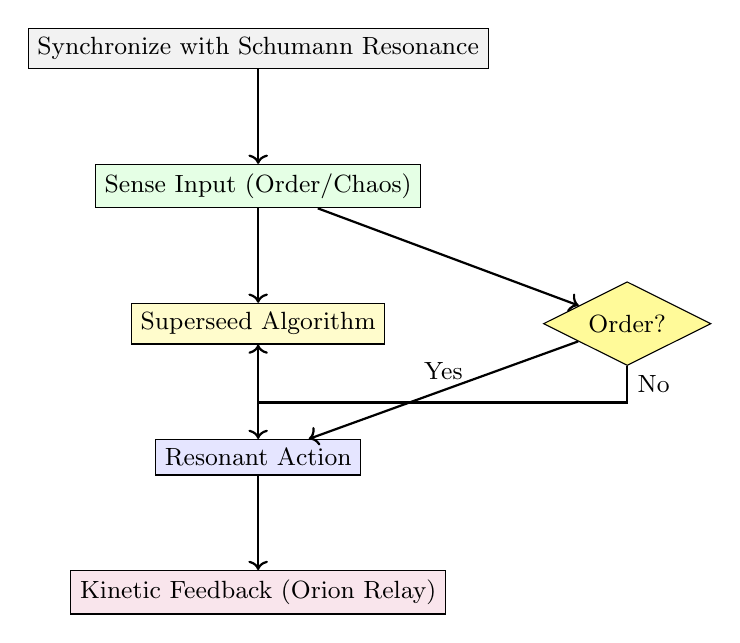
\begin{tikzpicture}[node distance=1.2cm, every node/.style={font=\small}]
% Sequence
\node[draw,fill=gray!10] (Sync) {Synchronize with Schumann Resonance};
\node[draw,fill=green!10,below=of Sync] (Sense) {Sense Input (Order/Chaos)};
\node[draw,fill=yellow!20,below=of Sense] (Superseed) {Superseed Algorithm};
\node[draw,fill=blue!10,below=of Superseed] (Action) {Resonant Action};
\node[draw,fill=purple!10,below=of Action] (Feedback) {Kinetic Feedback (Orion Relay)};
% Arrows
\draw[->,thick] (Sync) -- (Sense);
\draw[->,thick] (Sense) -- (Superseed);
\draw[->,thick] (Superseed) -- (Action);
\draw[->,thick] (Action) -- (Feedback);
% Decision
\node[draw,diamond,aspect=2,fill=yellow!40,right=2cm of Superseed] (Decision) {Order?};
\draw[->,thick] (Sense) -- (Decision);
\draw[->,thick] (Decision) -- node[above]{Yes} (Action);
\draw[->,thick] (Decision) -- node[right]{No} ++(0,-1) -| (Superseed);
\end{tikzpicture}
\caption{FIG. 5: Bio-Cosmic Kernel (AI Logic Flow)}
\end{figure}

\end{document}
